\section{鲁棒性 (健壮性)}

除了图\ref{fig:4.4} 中的直方图分析之外,Y. Pourasad等人还评估了输入图像和加密图像中两个垂直、
两个水平和两个对角相邻像素之间的相关性。 
图像中两个相邻像素的值由 x 轴和 y 轴表示。 
在输入图像和密码图像中,图\ref{fig:4.4}描绘了两个水平相邻像素的相关分布。 
普通图像和密码图像的相关系数分别为 0.99 和 0.02。 
对角线和垂直方向都产生相似的结果。 简单的图片具有两个相邻像素的高度相关性。

\begin{figure}[ht]
    \begin{center}
        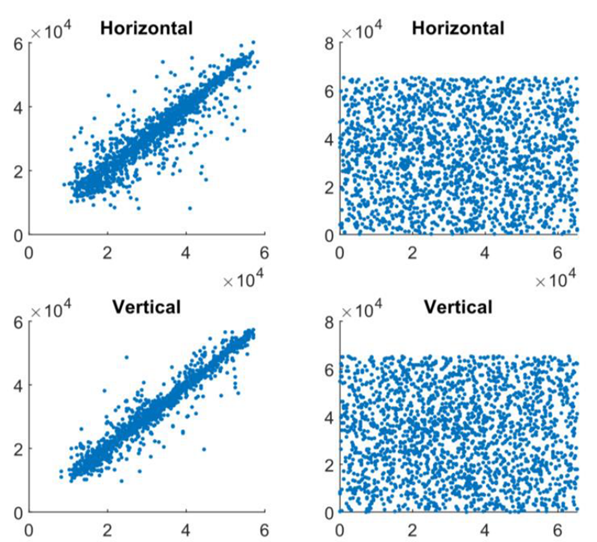
\includegraphics[width=\textwidth]{figure/p7.png}\\
        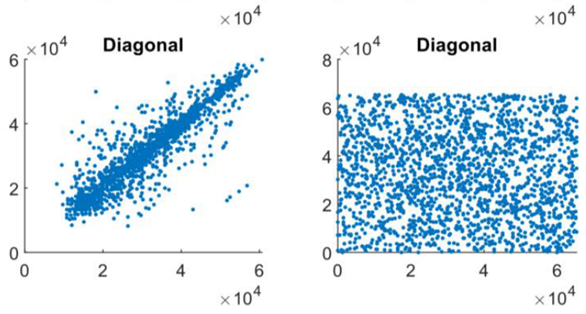
\includegraphics[width=\textwidth]{figure/p8.png}\\
    \end{center}
    \caption{Lena 图像中的像素水平、垂直和对角线、输入(左)和加密图像(右)的相关性图 \label{fig:4.4}}
\end{figure}

为了评估所提出的方法的鲁棒性,测试图像针对四种类型的图像处理攻击进行了测试:旋转、高斯噪声、中值过滤和直方图均衡。 
结果表明,所提出的设计具有更高的鲁棒性和归一化相关性。 根据结果,输入攻击不影响图像加解密。 关于不同类型图像的归
一化相关 (NC) 值,中值滤波器、旋转和高斯噪声具有更高的 NC 值。 这意味着所提出的方法的鲁棒性可以抵抗这些类型的攻
击。 然而,直方图均衡的影响是显着的(见表\ref{table:4.3})。\\

\begin{table}[ht]
    \wuhao
    \caption{所提算法在不同攻击类型下的 NC 值 \label{table:4.3}}
    \begin{tabularx}{\textwidth}{YYYYY}
        \Xhline{1.5pt}
        \bfseries Image & \bfseries Median Filter & \bfseries Histogram Equalization&\bfseries Rotation&\bfseries Gaussian Noise\\
        \Xhline{0.75pt}
        Lena & 0.984 & 0.987 & 0.999 & 0.999 \\
        Peppers & 0.704 & 0.280 & 0.923 & 0.964 \\
        Barbara & 0.914 & 0.497 & 0.980 & 0.991 \\
        Baloon & 0.960 & 0.629 & 0.991 & 0.996 \\
        Boat & 0.976 & 0.746 & 0.995 & 0.998 \\
        \Xhline{1.5pt}
    \end{tabularx}
\end{table}